%!TEX root = ../annotations.tex
\definecolor{lightgray}{gray}{0.96}
\newcommand*\rot{\rotatebox{90}}
\begin{document}
    \chapter{Introduction to agricultural robots}

    This report focuses on the problems in the development and deployment of agricultural robots and tries evaluate if system of multiple robots are able to bring advantages into this area.

    The global population is growing, at the same time the amount of arable land remains the same. Until 2050, the global population will surpass 9.1 billion people - which are going to mostly live in cities and are dependant on farmers fulfilling their steady demands to high quality foods. Even today, there are millions of people malnourished, with more even more people dependant on the limited food sources, this will get worse. \cite{FAO2021}
    
    Following the needs of more people, it will be important to grow even more food than currently obtainable. Because the existing land is limited, it is important to increase the efficiency of farming. 

    Not just the higher demand pressures farmers, but also another problem: Farming is highly dependant on human labour. Working in fields is demanding on the body and often detrimental for the health of the workers. Because of this, the available workforce shrinks by following other sectors of work instead. This makes quality work harder and harder to find for the farmers. \cite{Vasconez2019}

    Big scale conventional farming can of course produce high amounts of foods, but not without a hefty environmental footprint. Usage of pesticides and herbicides - often distributed blind over whole fields - is not sustainable and should be reduced if possible. \cite{ConesaMunoz2015}

    Those three points make already a convincing argument for automating the process of farming by robots - but why are our fields and greenhouses still taken care of by humans? 

    In contrast to modern industry, were factories work with minimal human labour and completely automated assembly lines, it seems that in agriculture some problem arise which still hinders the use of autonomous robots. 

    

    % Even though there are already fully automated factories and assembly lines, automations and robotics lack behind in the areas of agriculture. 
    % Because the there are no systems which are producing adequate results. 

    % The environment in which robots would have to work on fields are highly dynamic, unstructured, dirty, dust, highly stochastic \cite{Bechar2016}

    % There are some system which are able to do some task in open field tests, but even here is the performance too bad \cite{Bac2014}

    % In agriculture are many different tasks which need to be done, planting, scouting, plant care such as pruning, weed removal, and finally harvesting. 
    
    % Harvesting, what all is needed, sensing, processing the data, planning how to access the fruit, moving to the fruit and detaching it.  putting the fruit somewhere. This works okay with current technology as long as no leaves come between the cameras and the fruit. 
   
    % Most popular research topic is harvesting - even a robot fully capable of harvesting would not be used most of the year, because of the seasonality of the growth cycles.

    % All in all many problems hindering the adaption of automation in agriculture. 

    % It is Nevertheless an exiting field like all of field robots because of the need for automation here and the future potential in it. \cite{Thorpe2001}



    \chapter{Description of the subject}
        \section{Agricultural robots in the bigger field of robotic research.}

        One could divide the types of robotic applications into two main groups. First the group of \emph{industrial robots}, and second the group of \emph{service robots}. 
        Industrial robots are robots, which are used in the modern factories in highly automated scenarios. The \emph{International Standardization Organization} (ISO) defines them as "fixed in place or mobile for use in industrial automation application". 
        
        Service Robots on the other hand are defined by ISO as:
        \begin{displayquote}
            "Robot that performs useful tasks for humans or equipment excluding industrial automation applications."
        \end{displayquote} 

        Since this definition is still ambiguous, the ISO splits the field of service robots further into the two subfields of \emph{personal} and \emph{professional service robots}. \emph{Personal service robots} are robots used in non-commercial tasks by layman. Examples are robot vacuums, and general domestic servant robots. \emph{Professional service robots} in the other hand are the big field of robots used in commercial tasks by professionals.
        Now in the field of professional service robots, exists the category of \emph{field robots}. Field robots are defined by the Robotic Industries Association as:
        \begin{displayquote}
            "Field robots are non-factory mobile robots that operate in dynamic, unstructured environments. These types of robots aren’t programmed to repeat the same task over and over – they’re adaptive, responsive robots that work under variable conditions, sometimes even in unexplored territory. They often perform tasks that are too laborious or dangerous for humans. For this reason, as the underlying technology steadily advances their capabilities, field robots are becoming highly desirable to a number of different industries."
        \end{displayquote}

        Agricultural robots are a specific subfield of field robotics. They are indented to work in agricultural industry for the production of crops. 

        The field of agricultural robots is a subfield of field robotic. 

        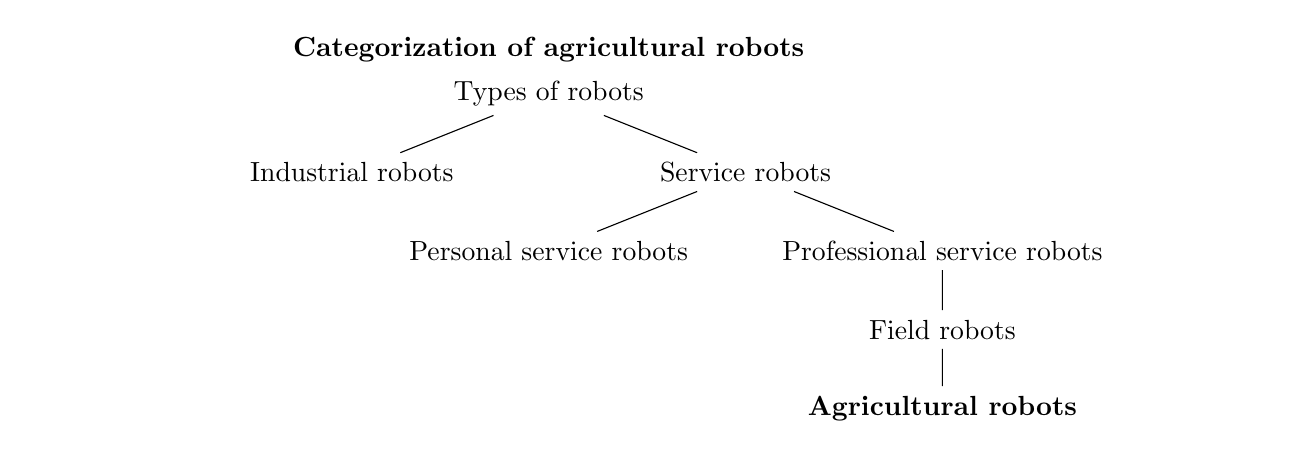
\begin{tikzpicture}[text width=8cm, align=flush center, level distance=1cm, sibling distance=5cm]
            \node[label=above:\textbf{Categorization of agricultural robots}]{Types of robots}
                child { node {Industrial robots}}
                child { node {Service robots}
                    child {node {Personal service robots}}
                    child {node {Professional service robots}
                        child {node {Field robots}
                            child {node {\textbf{Agricultural robots}}}
                        }
                    }
                }
            ;
        \label{fig:category_mindmap}
        \end{tikzpicture}

        \section{What makes the usage of robots in agriculture so hard?}

        \section{Can system with multiple robots help with the existing limitations?}


    \chapter{Description of the chosen papers}

    The biggest focus in this work lies at understanding the problems agricultural robots face, and second how MRS can help.

    \begin{table}[]
    \begin{tabular}{@{}llll@{}}
    \toprule
    Main topic            & Review paper                                                                                                & Broad use case                                                                                                               & Specific use case                                                                                                                     \\ \midrule
    Agricultural robotics & \begin{tabular}[c]{@{}l@{}}\hyperref[sec:Davidson2020]{Davidson2020}\\ \hyperref[sec:Bechar2016]{Bechar2016}\\ \hyperref[sec:Siciliano2016]{Siciliano2016}\\ \hyperref[sec:Zhao2016]{Zhao2016}\\ \hyperref[sec:Pedersen2006]{Pedersen2006}\end{tabular} & \begin{tabular}[c]{@{}l@{}}\hyperref[sec:deSantos2020]{deSantos2020}\\ \hyperref[sec:Vasconez2019]{Vasconez2019}\\ \hyperref[sec:deSantos2016]{deSantos2016}\\ \hyperref[sec:Roldan2016]{Roldan2016} \\ \hyperref[sec:ConesaMunoz2015]{ConesaMunoz2015}\\ \hyperref[sec:Bac2014]{Bac2014}\end{tabular} & \begin{tabular}[c]{@{}l@{}}\hyperref[sec:Arad2020]{Arad2020}\\ \hyperref[sec:Herck2020]{Herck2020}\\ \hyperref[sec:Lehnert2020]{Lehnert2020}\\ \hyperref[sec:Wu2020]{Wu2020}\\ \hyperref[sec:Albani2017]{Albani2017}\\ \hyperref[sec:Lili2017]{Lili2017}\\ \hyperref[sec:Weiss2011]{Weiss2011}\\ \hyperref[sec:Henten2003]{Henten2003}\end{tabular} \\
    Multi-robot systems   & \begin{tabular}[c]{@{}l@{}}\hyperref[sec:Khamis2015]{Khamis2015}\\ \hyperref[sec:Korsah2013]{Korsah2013}\\ \hyperref[sec:Lerman2006]{Lerman2006}\\ \hyperref[sec:Arai2002]{Arai2002}\\ \hyperref[sec:Gerkey2004]{Gerkey2004} \\ \hyperref[sec:Brambilla2013]{Brambilla2013}\end{tabular}        &  \hyperref[sec:Chamanbaz2017]{Chamanbaz2017}                                                                                                                      &                                                                                                                                      \\
    Field and service robotics & \begin{tabular}[c]{@{}l@{}} \hyperref[sec:Haidegger2013]{Haidegger2013} \\ \hyperref[sec:Thorpe2001]{Thorpe2001} \end{tabular}                                                                                               &                                                                                                                &                                                                                                                                      \\ \bottomrule
    \end{tabular}
    \label{table_topics}
    \end{table}

\begin{table}[]
    \rowcolors{1}{}{lightgray}
    \begin{tabular}{@{}lllllllllllllll@{}}
    \toprule
    Paper           & \rot{Review} & \rot{Agriculture} & \rot{MRS} & \rot{Swarm} & \rot{Field robotis} & \rot{Harvesting} & \rot{Scouting} & \rot{Weeding} & \rot{Communication} & \rot{Vision system} & \rot{Manipulation} & \rot{Simulation} & \rot{Lab experiment} & \rot{Field experiment} \\ \midrule
    \hyperref[sec:Albani2017]{Albani2017}      &        &  \checkmark          &  \checkmark  &  \checkmark    &  \checkmark            &            &  \checkmark       &  \checkmark      &  \checkmark            &  \checkmark            &              &  \checkmark         &                &                  \\
    \hyperref[sec:Albani2019]{Albani2019}      &        &  \checkmark          &  \checkmark  &  \checkmark    &  \checkmark            &            &  \checkmark       &  \checkmark      &  \checkmark            &  \checkmark            &              &  \checkmark         &  \checkmark             &                  \\
    \hyperref[sec:Arad2020]{Arad2020}        &        &  \checkmark          &     &       &  \checkmark            &  \checkmark         &          &         &               &  \checkmark            &  \checkmark           &            &                &  \checkmark               \\
    \hyperref[sec:Arai2002]{Arai2002}        &  \checkmark     &             &  \checkmark  &       &  \checkmark            &            &          &         &               &               &              &            &                &                  \\
    \hyperref[sec:Bac2014]{Bac2014}         &  \checkmark     &  \checkmark          &     &       &  \checkmark            &  \checkmark         &          &         &               &  \checkmark            &  \checkmark           &            &                &                  \\
    \hyperref[sec:Bechar2016]{Bechar2016}      &  \checkmark     &  \checkmark          &     &       &  \checkmark            &  \checkmark         &  \checkmark       &  \checkmark      &               &  \checkmark            &  \checkmark           &            &                &                  \\
    \hyperref[sec:Bechar2017]{Bechar2017}      &  \checkmark     &  \checkmark          &  \checkmark     &       &  \checkmark            &  \checkmark         &  \checkmark       &  \checkmark      &               &  \checkmark            &  \checkmark           &            &     \checkmark       &        \checkmark            \\
    \hyperref[sec:Brambilla2013]{Brambilla2013}   &  \checkmark     &             &  \checkmark  &  \checkmark    &               &            &          &         &  \checkmark            &               &              &            &                &                  \\
    \hyperref[sec:Chamanbaz2017]{Chamanbaz2017}   &        &             &  \checkmark  &  \checkmark    &  \checkmark            &            &          &         &  \checkmark            &  \checkmark            &              &  \checkmark         &  \checkmark             &  \checkmark               \\
    \hyperref[sec:ConesaMunoz2015]{ConesaMunoz2015} &        &  \checkmark          &  \checkmark  &       &  \checkmark            &            &          &  \checkmark      &  \checkmark            &  \checkmark            &              &            &  \checkmark             &  \checkmark               \\
    \hyperref[sec:Davidson2020]{Davidson2020}    &  \checkmark     &  \checkmark          &     &       &  \checkmark            &            &          &         &               &               &  \checkmark           &            &                &                  \\
    \hyperref[sec:deSantos2016]{deSantos2016}    &        &  \checkmark          &     &       &  \checkmark            &            &  \checkmark       &  \checkmark      &               &  \checkmark            &              &  \checkmark         &                &                  \\
    \hyperref[sec:deSantos2020]{deSantos2020}    &  \checkmark     &  \checkmark          &     &       &  \checkmark            &  \checkmark         &  \checkmark       &  \checkmark      &  \checkmark            &  \checkmark            &  \checkmark           &            &                &                  \\ 
    \hyperref[sec:Gerkey2004]{Gerkey2004}      &  \checkmark     &             &  \checkmark  &       &               &            &          &         &  \checkmark            &               &              &            &                &                  \\
    \hyperref[sec:Haidegger2013]{Haidegger2013}   &  \checkmark     &             &     &       &  \checkmark            &            &          &         &               &               &              &            &                &                  \\
    \hyperref[sec:Henten2003]{Henten2003}      &        &  \checkmark          &     &       &  \checkmark            &  \checkmark         &          &         &               &  \checkmark            &  \checkmark           &            &                &  \checkmark               \\
    \hyperref[sec:Herck2020]{Herck2020}      &        &  \checkmark          &     &       &  \checkmark            &  \checkmark         &          &         &               &  \checkmark            &  \checkmark           &            &                &  \checkmark               \\
    \hyperref[sec:Khamis2015]{Khamis2015}      &  \checkmark     &             &  \checkmark  &       &               &            &          &         &  \checkmark            &               &              &            &                &                  \\
    \hyperref[sec:Korsah2013]{Korsah2013}      &  \checkmark     &             &  \checkmark  &       &               &            &          &         &  \checkmark            &               &              &            &                &                  \\
    \hyperref[sec:Lehnert2020]{Lehnert2020}     &        &  \checkmark          &     &       &  \checkmark            &  \checkmark         &          &         &               &  \checkmark            &  \checkmark           &            &  \checkmark             &  \checkmark               \\
    \hyperref[sec:Lerman2006]{Lerman2006}      &        &             &  \checkmark  &       &               &            &          &         &  \checkmark            &               &              &            &                &                  \\
    \hyperref[sec:Lili2017]{Lili2017}        &        &  \checkmark          &     &       &  \checkmark            &  \checkmark         &          &         &               &  \checkmark            &              &            &                &  \checkmark               \\
    \hyperref[sec:Pedersen2006]{Pedersen2006}    &  \checkmark     &  \checkmark          &     &       &  \checkmark            &  \checkmark         &  \checkmark       &  \checkmark      &               &               &              &            &                &                  \\
    \hyperref[sec:Roldan2016]{Roldan2016}      &        &  \checkmark          &  \checkmark  &       &  \checkmark            &            &  \checkmark       &         &               &  \checkmark            &              &            &                &  \checkmark               \\
    \hyperref[sec:Siciliano2016]{Siciliano2016}   &  \checkmark     &  \checkmark          &     &       &  \checkmark            &  \checkmark         &  \checkmark       &  \checkmark      &               &  \checkmark            &  \checkmark           &            &                &  \checkmark               \\
    \hyperref[sec:Thorpe2001]{Thorpe2001}      &  \checkmark     &             &     &       &  \checkmark            &            &          &         &               &               &              &            &                &                  \\
    \hyperref[sec:Vasconez2019]{Vasconez2019}    &  \checkmark     &  \checkmark          &     &       &  \checkmark            &            &          &         &  \checkmark            &               &              &            &                &                  \\
    \hyperref[sec:Weiss2011]{Weiss2011}       &        &  \checkmark          &     &       &  \checkmark            &            &  \checkmark       &         &               &  \checkmark            &              &  \checkmark         &  \checkmark             &                  \\
    \hyperref[sec:Wu2020]{Wu2020}          &        &  \checkmark          &     &       &  \checkmark            &  \checkmark         &          &         &               &  \checkmark            &              &            &                &  \checkmark               \\
    \hyperref[sec:Zhao2016]{Zhao2016}        &  \checkmark     &  \checkmark          &     &       &  \checkmark            &  \checkmark         &          &         &               &  \checkmark            &              &            &                &                  \\ \bottomrule
    \end{tabular}
    \end{table}




\end{document}


